\documentclass[a4paper, 14pt]{extarticle}%тип документа

%Русский язык
\usepackage[T2A]{fontenc} %кодировка
\usepackage[utf8]{inputenc} %кодировка исходного кода
\usepackage[english,russian]{babel} %локализация и переносы

%отступы 
\usepackage[left=2cm,right=2cm,top=2cm,bottom=3cm,bindingoffset=0cm]{geometry}

%Вставка картинок
\usepackage{graphicx}
\usepackage{wrapfig, caption}
\graphicspath{}
\DeclareGraphicsExtensions{.pdf,.png,.jpg, .jpeg}
\newcommand\ECaption[1]{%
     \captionsetup{font=footnotesize}%
     \caption{#1}}

%Таблицы
\usepackage[table,xcdraw]{xcolor}
\usepackage{booktabs}

%Графики
\usepackage{pgfplots}
\pgfplotsset{compat=1.9}

%Математика
\usepackage{amsmath, amsfonts, amssymb, amsthm, mathtools}

%Заголовок
\author{Подлесный Артём \\ группа 827}
\title{Работа 150А \\ СПЕКТРАЛЬНЫЙ АНАЛИЗ ЭЛЕКТРИЧЕСКИХ СИГНАЛОВ}

\begin{document}
\maketitle
\paragraph*{Цель работы:}
В работе изучаются спектры периодических электрических сигналов
различной формы (последовательности прямоугольных импульсов и цугов,
а также амплитудно-модулированных гармонических колебаний). 
\paragraph*{Оборудование:} персональный компьютер; USB-осциллограф АКИП4107; функциональный генератор WaveStation 2012; соединительные кабели.
\section*{Экспериментальная установка}
\begin{figure}[h!]
\begin{center}
\includegraphics[width=0.8\textwidth]{ust}
\end{center}
\ECaption{Схема установки для проведения эксперимента.}
\end{figure}

Работа проводится на компьютере, поэтому единственное, что требуется для измерений - четко настраивать начальные параметры.

\section*{Исследование спектра периодической последовательности
прямоугольных импульсов.}

 Периодическая последовательность прямоугольных импульсов (рис. 2) с амплитудой $V_0$, длительностью $\tau$, частотой повторения $\Omega_1=2\pi/T$, где $Т$ — период повторения импульсов.
Найдём среднее значение (постоянную составляющую). Согласно формуле 
\[\left\langle V \right\rangle  = V_0\frac{\tau}{T}.\]
Коэффициенты при косинусовых составляющих равны:
\[a_n = 2V_0\frac{\tau}{T}\frac{\sin\left( \frac{n\Omega_1\tau}{2}\right) }{\frac{n\Omega_1\tau}{2}} \sim \frac{\sin x}{x}.\]

Поскольку наша функция чётная, все коэффициенты синусоидальных гармоник равны 0. Спектр $a_n$ последовательности прямоугольных импульсов представлен на рис. 2. 

\begin{figure}[h!]
\begin{center}
\includegraphics[width=0.8\textwidth]{a}
\end{center}
\ECaption{Слева -- периодическая
последовательность	
прямоугольных импульсов, справа  --  её спектр.}
\end{figure}
 
Здесь видна ширина спектра $\Delta \nu$. 

После установки всех необходимых параметров, получаем картину спектра.
Можно понять, как он меняется в зависимости от $f_{\text{повт}}$ и $\tau$. Для этого они поочередно изменялись в 2 раза, что показано на рис. 3. Отсюда подтверждаем, что $\tau\Delta\nu \sim 1$.  

\begin{figure}[h!]
\begin{center}
\includegraphics[width=0.6\textwidth]{spec}
\end{center}
\ECaption{Картина спектра: сверху рабочий спектр, под ним - спектр  с увеличенной вдвое $\tau$ и неизменной частотой $f_{\text{повт}}$, ниже -  спектр  с увеличенной вдвое $f_{\text{повт}}$ и неизменной $\tau$. }
\end{figure}

Далее были проведены измерения зависимости ширины спектра от длительности импульса, представленные на таблице 1.

\begin{table}[h]
\begin{center}
\begin{tabular}{|c|c|c|c|c|c|c|c|c|c|}
\hline
\rowcolor[HTML]{9698ED} 
$\Delta\nu$, кГц & 24 & 16 & 11 & 9.6 & 8.2 & 7   & 6.1 & 5.6 & 4.8 \\ \hline
$\tau$, мкс      & 40 & 60 & 80 & 100 & 120 & 140 & 160 & 180 & 200 \\ \hline
\end{tabular}

\end{center}
\ECaption{Данные зависимости $\Delta\nu(\tau)$. }
\end{table} 

Далее в работе необходимо было посчитать зависимость между номером гармоники спектра, амплитудой и частотой этой гармоники, при начальной частоте $f = 1$ кГц, и $\tau = 50 $, и 100 мкс. Благодаря точности установки, частоты совпадали с номером гармоники в кГц, что не удивительно с таким значением частоты. Данные представлены на таблице 2, а картины самих спектров представлены на рис. 4. 



\begin{table}[h!]
\begin{center}
\begin{tabular}{|c|c|c|ccc}
\hline
50 мкс                     &                               &                               & \multicolumn{1}{c|}{100 мкс}                   & \multicolumn{1}{c|}{}                              & \multicolumn{1}{c|}{}                                 \\ \hline
\rowcolor[HTML]{9698ED} 
$n$                          & $A$, мВ                         & $\nu$, кГц                      & \multicolumn{1}{c|}{\cellcolor[HTML]{9698ED}$n$} & \multicolumn{1}{c|}{\cellcolor[HTML]{9698ED}$A$, мВ} & \multicolumn{1}{c|}{\cellcolor[HTML]{9698ED}$\nu$, кГц} \\ \hline
0                          & 123.5                         & 0.003                         & \multicolumn{1}{c|}{0}                         & \multicolumn{1}{c|}{221.4}                         & \multicolumn{1}{c|}{0.001}                            \\ \hline
\rowcolor[HTML]{9698ED} 
1                          & 68.97                         & 1.005                         & \multicolumn{1}{c|}{\cellcolor[HTML]{9698ED}1} & \multicolumn{1}{c|}{\cellcolor[HTML]{9698ED}136.5} & \multicolumn{1}{c|}{\cellcolor[HTML]{9698ED}1.002}    \\ \hline
2                          & 66.76                         & 2.003                         & \multicolumn{1}{c|}{2}                         & \multicolumn{1}{c|}{127.1}                         & \multicolumn{1}{c|}{2.005}                            \\ \hline
\rowcolor[HTML]{9698ED} 
3                          & 63.18                         & 3.004                         & \multicolumn{1}{c|}{\cellcolor[HTML]{9698ED}3} & \multicolumn{1}{c|}{\cellcolor[HTML]{9698ED}113.1} & \multicolumn{1}{c|}{\cellcolor[HTML]{9698ED}2.996}    \\ \hline
4                          & 58.53                         & 4.004                         & \multicolumn{1}{c|}{4}                         & \multicolumn{1}{c|}{94.9}                          & \multicolumn{1}{c|}{4.021}                            \\ \hline
\rowcolor[HTML]{9698ED} 
5                          & 57.1                          & 4.997                         & \multicolumn{1}{c|}{\cellcolor[HTML]{9698ED}5} & \multicolumn{1}{c|}{\cellcolor[HTML]{9698ED}80.72} & \multicolumn{1}{c|}{\cellcolor[HTML]{9698ED}5.002}    \\ \hline
6                          & 57.01                         & 5.997                         & \multicolumn{1}{c|}{6}                         & \multicolumn{1}{c|}{66.76}                         & \multicolumn{1}{c|}{5.994}                            \\ \hline
\rowcolor[HTML]{9698ED} 
7                          & 55.2                          & 6.999                         & \multicolumn{1}{c|}{\cellcolor[HTML]{9698ED}7} & \multicolumn{1}{c|}{\cellcolor[HTML]{9698ED}50.3}  & \multicolumn{1}{c|}{\cellcolor[HTML]{9698ED}7.008}    \\ \hline
8                          & 52.45                         & 7.999                         & \multicolumn{1}{c|}{8}                         & \multicolumn{1}{c|}{32.38}                         & \multicolumn{1}{c|}{8.01}                             \\ \hline
\cellcolor[HTML]{9698ED}9  & \cellcolor[HTML]{9698ED}48.75 & \cellcolor[HTML]{9698ED}9.002 &                                                &                                                    &                                                       \\ \cline{1-3}
10                         & 43.81                         & 10                            &                                                &                                                    &                                                       \\ \cline{1-3}
\cellcolor[HTML]{9698ED}11 & \cellcolor[HTML]{9698ED}38.59 & \cellcolor[HTML]{9698ED}11    &                                                &                                                    &                                                       \\ \cline{1-3}
12                         & 32.89                         & 12                            &                                                &                                                    &                                                       \\ \cline{1-3}
\cellcolor[HTML]{9698ED}13 & \cellcolor[HTML]{9698ED}27.06 & \cellcolor[HTML]{9698ED}13.01 &                                                &                                                    &                                                       \\ \cline{1-3}
14                         & 23.87                         & 13.99                         &                                                &                                                    &                                                       \\ \cline{1-3}
\cellcolor[HTML]{9698ED}15 & \cellcolor[HTML]{9698ED}20.32 & \cellcolor[HTML]{9698ED}15    &                                                &                                                    &                                                       \\ \cline{1-3}
\end{tabular}
\ECaption{Таблица значений амплитуд для 2 спектров, с длительностью импульса в 50 и 100 мкс соответственно. }
\end{center}
\end{table}

\begin{figure}[h!]
\begin{center}
\includegraphics[width=0.8\textwidth]{speca}
\end{center}
\ECaption{Спектры прямоугольных импульсов, где слева длительность импульса -- 50 мкс, справа -- 100 мкс.}
\end{figure}

Построим график $\Delta\nu(\frac{1}{\tau})$. Он показан на рисунке 5.

\begin{figure}[h!]
\begin{center}
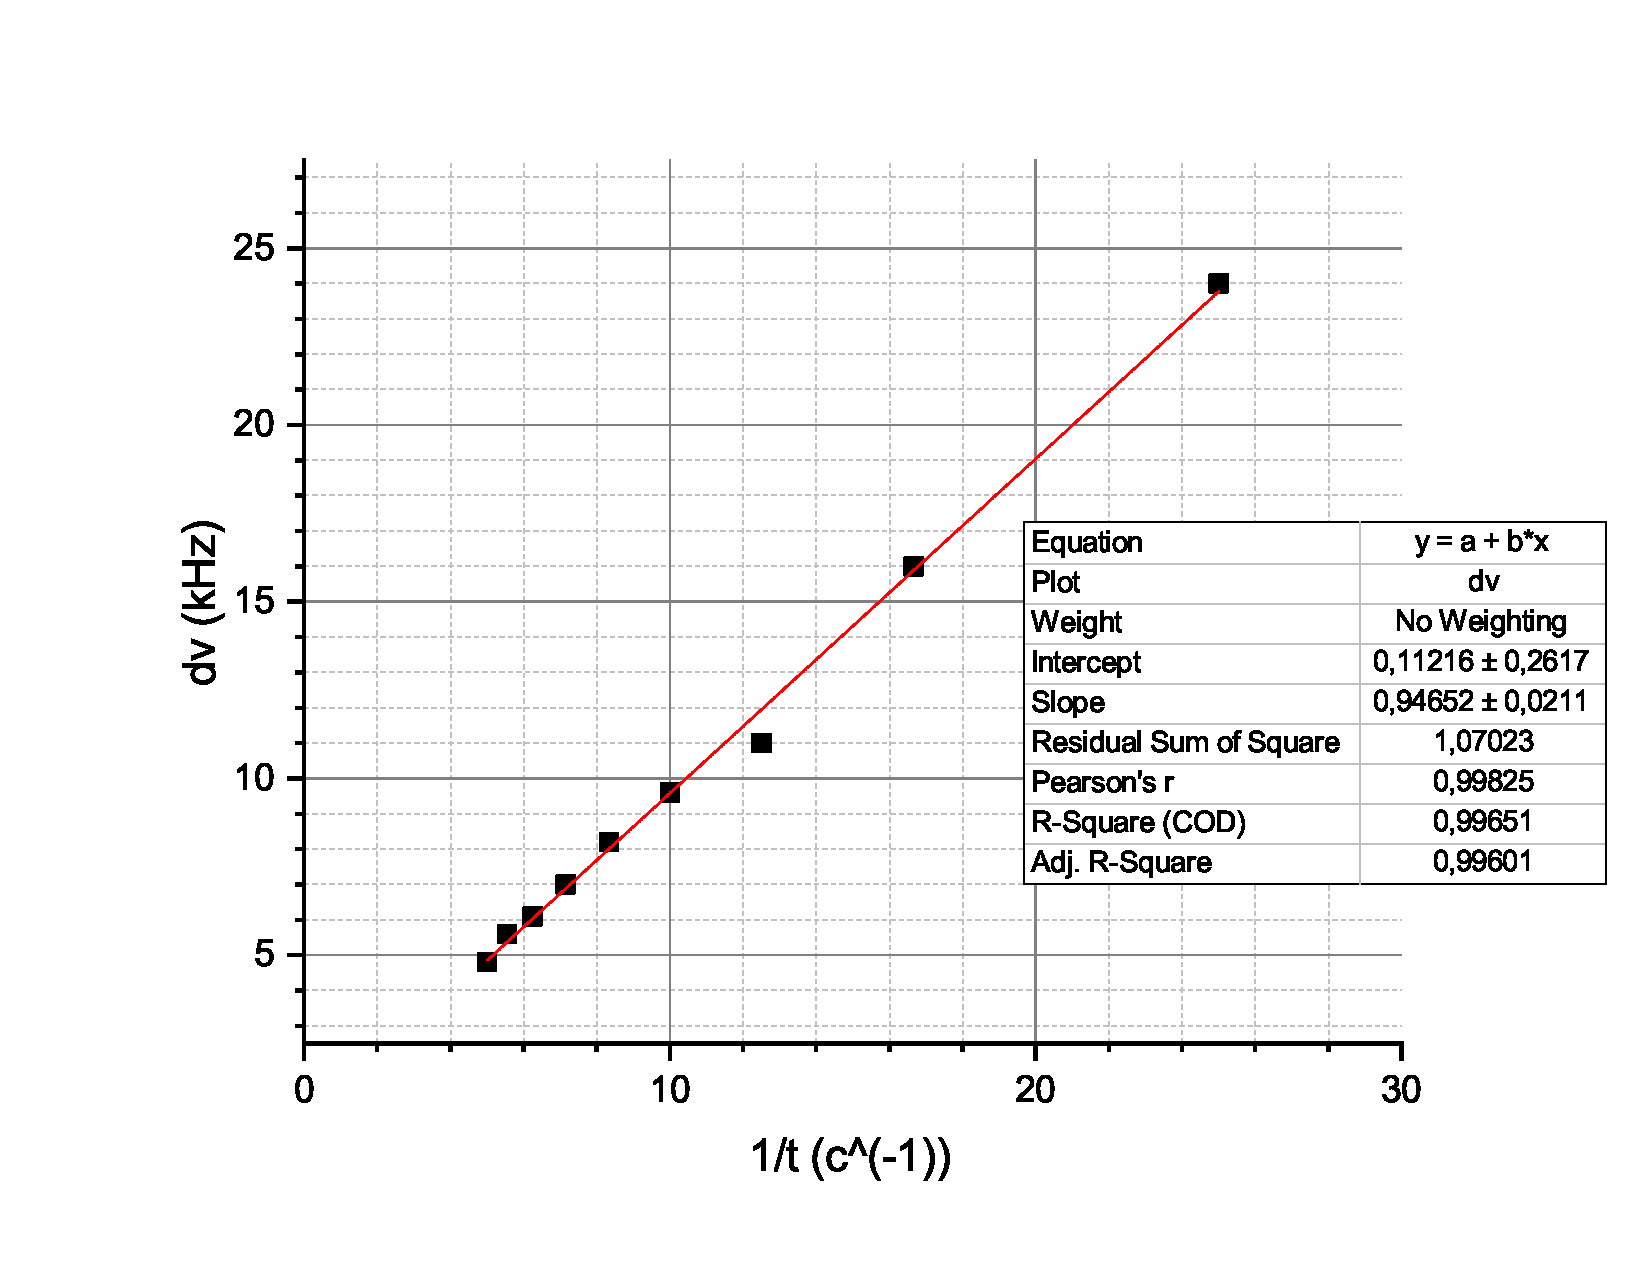
\includegraphics[width=1\textwidth]{grvt}
\end{center}
\ECaption{График зависимости $\Delta\nu(\frac{1}{\tau})$, показывающий выполнение частного случая принципа неопределенности.}
\end{figure}



\subsection*{Вывод}

Как видно по графику, его угол наклона - 0.95, а точка пересечения с осью ординат - 0.1, что показывает, что он практически проходит через начало координат. На основании этого можем убедиться в том, что соотношение неопределенности $\Delta\nu\Delta t \simeq 1$ -- выполняется. Несовместимость острой локализации волнового процесса во времени с узким спектром частот — явление широко известное в радиотехнике. Ширина селективной настройки $\Delta\nu$ радиоприёмника ограничивает приём радиосигналов длительностью $t < 1/\Delta\nu$. 

По картинам спектра так же заметно это соотношение, к тому же амплитуды импульсов спектра с большей их длительностью -- выше, что логично. 
\newpage 

\section*{Исследование спектра периодической последовательности
цугов гармонических колебаний.}
Периодическая последовательность цугов гармонического колебания $V_0\cos(\omega_0t)$ с длительностью цуга $\tau$ и периодом повторения $T$ (рис. 6).

\begin{figure}[h!]
\begin{center}
\includegraphics[width=0.8\textwidth]{b}
\end{center}
\ECaption{Слева -- периодическая
последовательность	
цугов, справа  --  её спектр.}
\end{figure}

Коэффициент при $n$-й гармонике согласно формуле равен:
\[a_n = V_0\frac{\tau}{T}\left( \dfrac{\sin[(\omega_0-n\Omega_1)\frac{\tau}{2}]}{(\omega_0-n\Omega_1)\frac{\tau}{2}} + \dfrac{\sin[(\omega_0+n\Omega_1)\frac{\tau}{2}]}{(\omega_0+n\Omega_1)\frac{\tau}{2}}   \right) .\]
Спектр на рис. 6 соответствует случаю, когда $T/\tau$ -- целое число.

После всех приготовлений получаем картину спектра периодических цуг (рис. 7).

\begin{figure}[h!]
\begin{center}
\includegraphics[width=1\textwidth]{cy}
\end{center}
\ECaption{Cпектр цуг -- слева при длительности импульса в 100 мкс, справа - в 200.}
\end{figure}

Несущая частоты в эксперименте - 30 кГц, определяла то, в каком месте спектра главный пик. При уменьшении/увеличении нес частоты, он смещался в лево/право.

Далее по работе была снята зависимость между $\delta\nu$ и $f_{\text{повт}}$. Она показана на таблице 3.

\begin{table}[h!]
\begin{center}
\begin{tabular}{|c|c|c|c|c|}
\hline
\rowcolor[HTML]{9698ED} 
$\delta\nu$       & 1.004 & 0.5 & 2 & 4 \\ \hline
$f_{\text{повт}}$ & 1     & 0.5 & 2 & 4 \\ \hline
\end{tabular}
\ECaption{Зависимость между $\delta\nu$ и $f_{\text{повт}}$.}
\end{center}
\end{table}

Как видно, необязательно даже строить график, чтобы понять, что его угол наклона будет 1, и $f_{\text{гармоники-n}} = nf_{\text{повт}}$.

Как и для прямоугольных импульсов, для цуг была снята зависимость амплитуды гармоники от её номера, по которым были восстановлены спектры для двух начальных условий: при начальной частоте $f = 1$ и 2 кГц, и $\tau = 100 $  мкс. Данные представлены на таблице 4, а сами спектры - на рис. 8.

\begin{table}[h!]
\begin{center}
\begin{tabular}{|c|c|cc}
\hline
1 кГц                     &                               & \multicolumn{1}{c|}{2 кГц}                       & \multicolumn{1}{c|}{}                                \\ \hline
\rowcolor[HTML]{9698ED} 
$n$                       & $A$, мВ                       & \multicolumn{1}{c|}{\cellcolor[HTML]{9698ED}$n$} & \multicolumn{1}{c|}{\cellcolor[HTML]{9698ED}$A$, мВ} \\ \hline
0                         & 73.34                         & \multicolumn{1}{c|}{0}                           & \multicolumn{1}{c|}{130.8}                           \\ \hline
\rowcolor[HTML]{9698ED} 
1                         & 56.25                         & \multicolumn{1}{c|}{\cellcolor[HTML]{9698ED}1}   & \multicolumn{1}{c|}{\cellcolor[HTML]{9698ED}107.3}   \\ \hline
2                         & 53.4                          & \multicolumn{1}{c|}{2}                           & \multicolumn{1}{c|}{85.44}                           \\ \hline
\rowcolor[HTML]{9698ED} 
3                         & 49.13                         & \multicolumn{1}{c|}{\cellcolor[HTML]{9698ED}3}   & \multicolumn{1}{c|}{\cellcolor[HTML]{9698ED}55.63}   \\ \hline
4                         & 42.84                         & \multicolumn{1}{c|}{4}                           & \multicolumn{1}{c|}{24.68}                           \\ \hline
\rowcolor[HTML]{9698ED} 
5                         & 35.6                          & \multicolumn{1}{c|}{\cellcolor[HTML]{9698ED}5}   & \multicolumn{1}{c|}{\cellcolor[HTML]{9698ED}5.317}   \\ \hline
6                         & 27.89                         &                                                  &                                                      \\ \cline{1-2}
\cellcolor[HTML]{9698ED}7 & \cellcolor[HTML]{9698ED}20.06 &                                                  &                                                      \\ \cline{1-2}
8                         & 12.46                         &                                                  &                                                      \\ \cline{1-2}
\cellcolor[HTML]{9698ED}9 & \cellcolor[HTML]{9698ED}5.578 &                                                  &                                                      \\ \cline{1-2}
10                        & 2.611                         &                                                  &                                                      \\ \cline{1-2}
\end{tabular}
\ECaption{Таблица данных гармоник спектра.}
\end{center}
\end{table}


\begin{figure}[h!]
\begin{center}
\includegraphics[width=0.5\textwidth]{specb}
\end{center}
\ECaption{Экспериментальные пектры цуг -- слева при частоте повтора в 1 кГц, справа -- 2.}
\end{figure}
\newpage
\subsection*{Вывод}

Как видно из спектров цуг - при увеличении частоты повтора число гармоник уменьшается, а амплитуда увеличивается, что вполне согласуется с теорией. Так же можно увидеть, что в отличие от прямоугольных импульсов, положение главной гармоники определяет еще и несущая частота, когда как прямоугольные импульсы имеют максимум амплитуды в нуле.
Так же заметно, что амплитуда прямоугольных импульсов - больше.

\section*{Исследование спектра гармонических сигналов,
модулированных по амплитуде}

Амплитудно-модулированные колебания задаются формулой:
\[f(t) = A_0(1+m\cos\Omega t)\cos\omega_0t.\]
Коэффициент $m$ называют глубиной модуляции. Глубина модуляции может быть представлена в виде:
\[m = \dfrac{A_{max}-A_{min}}{A_{max}+A_{min}}.\]
Такие колебания легко разложить по спектру:
\begin{equation}
f(t) = A_0\cos\omega_0t + \frac{A_0m}{2}\cos(\omega_0+\Omega)t+ \frac{A_0m}{2}\cos(\omega_0-\Omega)t.
\end{equation}

Они показаны на рис. 9.

\begin{figure}[h!]
\begin{center}
\includegraphics[width=0.8\textwidth]{m}
\end{center}
\ECaption{Амплитудно-модулированные колебания и их спектр.}
\end{figure}

В работе были измерены значения всех амплитуд, в зависимости от двойного напряжения входящего сигнала. Тогда для каждого из значений Vpp была посчитана глубина модуляции сигнала. Эти данные представлены таблицей 5.

\begin{table}[h!]
\begin{center}
\begin{tabular}{|c|c|c|c|c|c|}
\hline
\rowcolor[HTML]{9698ED} 
Ampl, Vpp & $A_{max}$ & $A_{min}$ & $A_{\text{осн}}$ & $A_{\text{бок}}$ & $m$   \\ \hline
0.2       & 545.6     & 456       & 326.4            & 14.47            & 0.089 \\ \hline
\rowcolor[HTML]{9698ED} 
0.5       & 625       & 379.2     & 326.4            & 39.62            & 0.245 \\ \hline
0.8       & 694.2     & 310       & 326.4            & 61.14            & 0.383 \\ \hline
\rowcolor[HTML]{9698ED} 
1.1       & 773.6     & 238.3     & 328              & 84.87            & 0.529 \\ \hline
1.4       & 850.4     & 159       & 327.8            & 110.9            & 0.685 \\ \hline
\rowcolor[HTML]{9698ED} 
1.7       & 922.1     & 79.58     & 326.6            & 130.5            & 0.841 \\ \hline
2         & 988       & 98.11     & 353.9            & 139.7            & 0.819 \\ \hline
\end{tabular}
\ECaption{Различные амплитуды ам-колебаний. Для каждого сигнала посчитана его глубина модуляции.}
\end{center}
\end{table}

Так же теперь мы можем посмотреть, как меняется картина колебаний при увеличении $\Omega$. Это показано на рис. 10. 

\begin{figure}[h!]
\begin{center}
\includegraphics[width=0.8\textwidth]{m0}
\end{center}
\ECaption{Сверху вниз -- изменение картины ам-колебаний при увеличении $\Omega$ в 2 раза. Как видно, при этом уменьшается период колебаний амплитуды, что согласуется с теорией.}
\end{figure}

Из теории 
\[\frac{A_{\text{бок}}}{A_{\text{осн}}} = \frac{m}{2}.\]
Соответственно, угловой коэффициент графика зависимости $\frac{A_{\text{бок}}}{A_{\text{осн}}}(m)$ должен быть равен 0.5. Проверим это, построив график, изображенный на рис.11.

\begin{figure}[h!]
\begin{center}
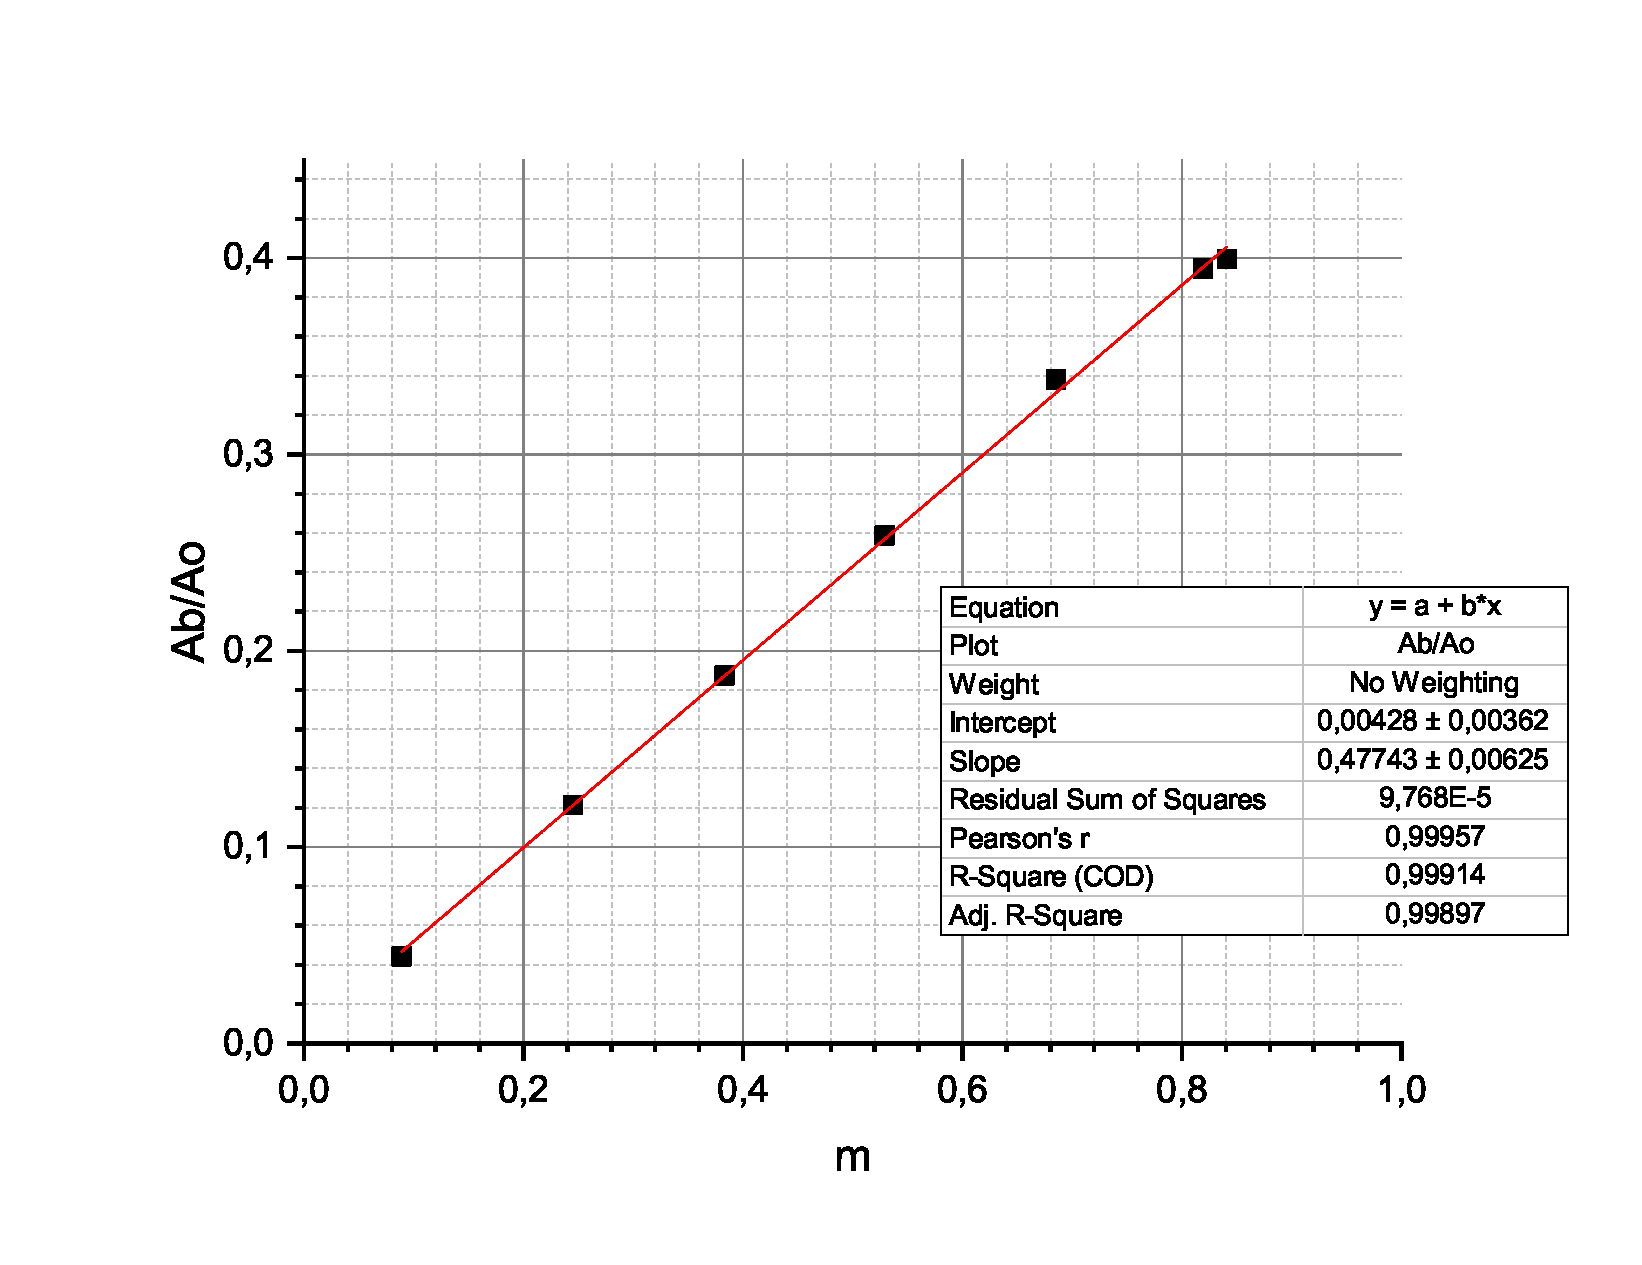
\includegraphics[width=0.8\textwidth]{grm}
\end{center}
\ECaption{График зависимости $\frac{A_{\text{бок}}}{A_{\text{осн}}}(m)$.}
\end{figure}

\subsection*{Вывод}

Как видно из графика, его коэффициент наклона 0.47, что примерно равно 0.5, поэтому колебательный режим можно действительно считать амплитудно-модулированным, а его спектр действительно задается функцией (1). 







\end{document}
